\documentclass[runningheads]{llncs}

\usepackage[utf8]{inputenc}
\usepackage{graphicx}
\usepackage{amsmath,amssymb}
\usepackage{booktabs}
\usepackage{siunitx}
\usepackage{xcolor}
\usepackage{algorithm}
\usepackage{algpseudocode}
\usepackage[hidelinks,bookmarks=false,pdfusetitle]{hyperref}
\usepackage[capitalise,noabbrev]{cleveref}
\usepackage{microtype}

\setcounter{tocdepth}{2}
\setcounter{secnumdepth}{3}

\sisetup{detect-all=true,group-separator={,},round-mode=places,round-precision=4,round-pad=false}

\title{Modern Portfolio Theory and\\
Risk-Adjusted Optimisation\\
\vspace{0.4em}
\large MSDM5058 Project~II}

\author{ZHAO Fuxian}
\titlerunning{Modern Portfolio Theory and Risk-Adjusted Optimisation}
\authorrunning{ZHAO Fuxian}
\institute{HKUST -- Information Science MSc Programme\\
MSDM5058 Information Science -- Spring 2026}

\begin{document}
\maketitle
\thispagestyle{empty}
\newpage

\begin{abstract}
The Markowitz tangency portfolio is a textbook winner in two assets
and a textbook victim of estimation error in six. On the
\textsc{aal}/\textsc{dal}/\textsc{spy}/\textsc{qqq}/\textsc{xlk}/\textsc{tnx}
panel observed 2008-01-02 to 2026-03-31 ($N{=}\num{4587}$ return
observations, $3{:}1$ split at $t_{0}{=}\,$2021-09-02), the unconstrained
tangency portfolio recommends roughly $2.1\!\times$ gross leverage in-sample
and immediately loses out-of-sample, while a risk-parity allocation
that uses none of the noisy mean vector $\hat\mu$ closes the future
window with Sharpe $\num{0.54}$, Calmar $\num{0.35}$ and maximum
drawdown $-21.9\%$ versus $-59.3\%$ for buy-and-hold AAL. Five
further estimators are layered on the basic frontier --- CAPM
decomposing each asset into market beta and idiosyncratic alpha,
Black-Litterman shrinking $\hat\mu$ toward the CAPM-implied prior,
multi-asset Kelly and a half-Kelly variant, and CVaR/ES at the $5\%$
and $1\%$ tails --- and a $15\%$-annualised vol-target overlay places
the four MPT strategies on a common ex-ante budget for honest
out-of-sample comparison. All optimisations scale as $O(K^{3})$ in
the asset count.
\keywords{Mean-Variance Analysis \and CAPM \and Black-Litterman \and
Kelly Criterion \and CVaR \and Risk Parity \and Vol Targeting.}
\end{abstract}
\newpage

\tableofcontents
\newpage

% =====================================================================
\section{Introduction}\label{sec:intro}
% =====================================================================
The Markowitz mean--variance frontier~\cite{markowitz1952} is the
canonical starting point of portfolio theory and the canonical victim
of estimation error. In a two-asset universe the conditioning of
$\hat\Sigma$ is benign and the tangency weights are trustworthy; in a
six-asset universe the same closed form recommends $3.7\!\times$
gross leverage and short-side exposure that the textbook politely
ignores --- the well-documented Michaud
enigma~\cite{michaud1989}. The diagnostic is sharp on the
\textsc{aal}/\textsc{dal}/\textsc{spy}/\textsc{qqq}/\textsc{xlk}/\textsc{tnx}
panel observed 2008-01-02 to 2026-03-31 ($N{=}\num{4587}$ return
observations, $3{:}1$ split at $t_0{=}\,$2021-09-02): the unconstrained
tangency portfolio attains a past-window Sharpe of
$\num{0.84}$~\cite{sharpe1966} and immediately loses out-of-sample,
while a risk-parity allocation~\cite{maillard2010} that uses none of
the noisy mean vector $\hat\mu$ closes the future window with Sharpe
$\num{0.54}$, Calmar $\num{0.35}$ and a maximum drawdown of
$-21.9\%$ versus $-59.3\%$ for buy-and-hold AAL. The estimator that
spends the least information wins.

This paper layers five further estimators on the basic frontier, each
addressing a specific failure mode of plain Markowitz.
CAPM~\cite{sharpe1964capm,lintner1965} regressions versus SPY
decompose each asset into market beta and idiosyncratic alpha,
locating the largest positive CAPM alpha on QQQ ($+5.5\%$,
$\beta\!\approx\!0.99$), while both airlines load with $\beta>1.3$
but exhibit negative point estimates for $\alpha$. Black--Litterman~\cite{black1992,he1999bl}
treats the CAPM-implied equilibrium returns
$\Pi=\delta\Sigma w_{\mathrm{mkt}}$ as a prior and tilts it with a
single Bayes-derived directional view
($\textsc{aal}{-}\textsc{dal}>{+}5\%$), shrinking $\hat\mu$
rather than trusting it. The Kelly criterion~\cite{kelly1956}
delivers growth-optimal sizing
$w^{\star}=\Sigma^{-1}(\mu-r_f\mathbf{1})$ and we report a half-Kelly
variant alongside it as a catastrophe-bounded sibling.
CVaR/ES~\cite{rockafellar2000} at the $5\%$ and $1\%$ tails exposes
the concentration that variance hides --- single-asset \textsc{tnx}
carries the heaviest $1\%$-tail per unit variance, which is why an
equal-weighted portfolio under-performs the risk-parity weights that
scale \textsc{tnx} down. Risk parity itself is the structural
opposite of tangency: it enforces equal marginal risk contribution
and uses none of $\hat\mu$, hence its robustness when $\hat\mu$ is
the noisy input.

A $15\%$-annualised vol-target overlay places the four MPT
strategies (tangency, risk-parity, Black-Litterman, half-Kelly) on a
common ex-ante budget so that out-of-sample comparison is meaningful.
Risk-parity wins on every risk-adjusted metric, half-Kelly mirrors
tangency at half the leverage, and Black-Litterman recovers most of
the unconstrained-tangency loss by shrinking $\hat\mu$ toward the
equilibrium prior. The remainder of the paper develops the data and
the unconstrained and long-only Markowitz frontiers, the CAPM
regressions, the Black-Litterman tilt, Kelly sizing, the CVaR
analysis, risk-parity weights, the marginal and Bayes-detector
diagnostics, and the trading simulator under the vol-target overlay.

% =====================================================================
\section{Data Preprocessing}\label{sec:data}
% =====================================================================
The shared panel contains daily auto-adjusted close prices for nine
tickers over 2008-01-02 to 2026-03-31. We work on the six-asset subset
$\{\textsc{aal},\textsc{dal},\textsc{spy},\textsc{qqq},\textsc{xlk},
\textsc{tnx}\}$ and use log returns
$x_{i,t}=\ln(P_{i,t}/P_{i,t-1})$. The split point
$t_{0}{=}\,$2021-09-02 (75\%/25\% past:future) gives
$n_{\text{past}}{=}\num{3439}$ and
$n_{\text{fut}}{=}\num{1148}$ daily observations. \Cref{tab:moments} reports
annualised first and second moments on the past window.
\begin{table}[!htbp]
\centering\small
\caption{Past-window annualised moments (six-asset universe).}\label{tab:moments}
\begin{tabular}{lS[round-precision=4]S[round-precision=4]}
\toprule
Ticker & {Ann. mean} & {Ann. std-dev}\\
\midrule
AAL & 0.0328 & 0.6975\\
DAL & 0.0874 & 0.5418\\
SPY  & 0.1032 & 0.2064\\
QQQ  & 0.1571 & 0.2225\\
XLK  & 0.1475 & 0.2284\\
TNX  & -0.0804 & 0.4662\\
\bottomrule
\end{tabular}
\end{table}

% =====================================================================
\section{Mean-Variance Analysis and the Markowitz Frontier}\label{sec:mva}
% =====================================================================
\subsection{Closed-form unconstrained solution}
For a $K$-asset universe with mean vector $\mu$ and covariance
$\Sigma$, the unconstrained variance-minimising portfolio achieving a
target return $\mu_{T}$ has weights
\begin{equation}
w(\mu_T)=\Sigma^{-1}\!\bigl(\lambda\mathbf{1}+\gamma\mu\bigr),
\qquad
\begin{aligned}
\lambda&=(C-\mu_T B)/\Delta,\\
\gamma&=(\mu_T A-B)/\Delta,
\end{aligned}
\label{eq:frontier}
\end{equation}
with $A{=}\mathbf{1}^{\top}\Sigma^{-1}\mathbf{1}$, $B{=}\mathbf{1}^{\top}\Sigma^{-1}\mu$,
$C{=}\mu^{\top}\Sigma^{-1}\mu$, $\Delta{=}AC-B^{2}$. The minimum-variance
portfolio is recovered at $\mu_T{=}B/A$, the tangency portfolio at
$\mu_{T}^{*}{=}(C-B r_{f})/(B-A r_{f})$.

\subsection{Long-only solution by SLSQP}
The long-only frontier solves
$\min_{w}w^{\top}\Sigma w$ subject to $\mathbf{1}^{\top}w{=}1$, $w^{\top}\mu{=}\mu_{T}$,
$w_{i}\ge 0$. We solve this with sequential least-squares programming
(SLSQP) on the same $\mu_{T}$ grid; the result is plotted in
\cref{fig:front}. The unconstrained tangency portfolio has Sharpe
\num{0.84} but concentrates long exposure in QQQ while shorting
AAL, SPY, XLK and \textsc{tnx}; the long-only
front\-ier truncates these and yields a noticeably lower
Sharpe ($\!\sim\!0.51$).
\begin{figure}[!htbp]
\centering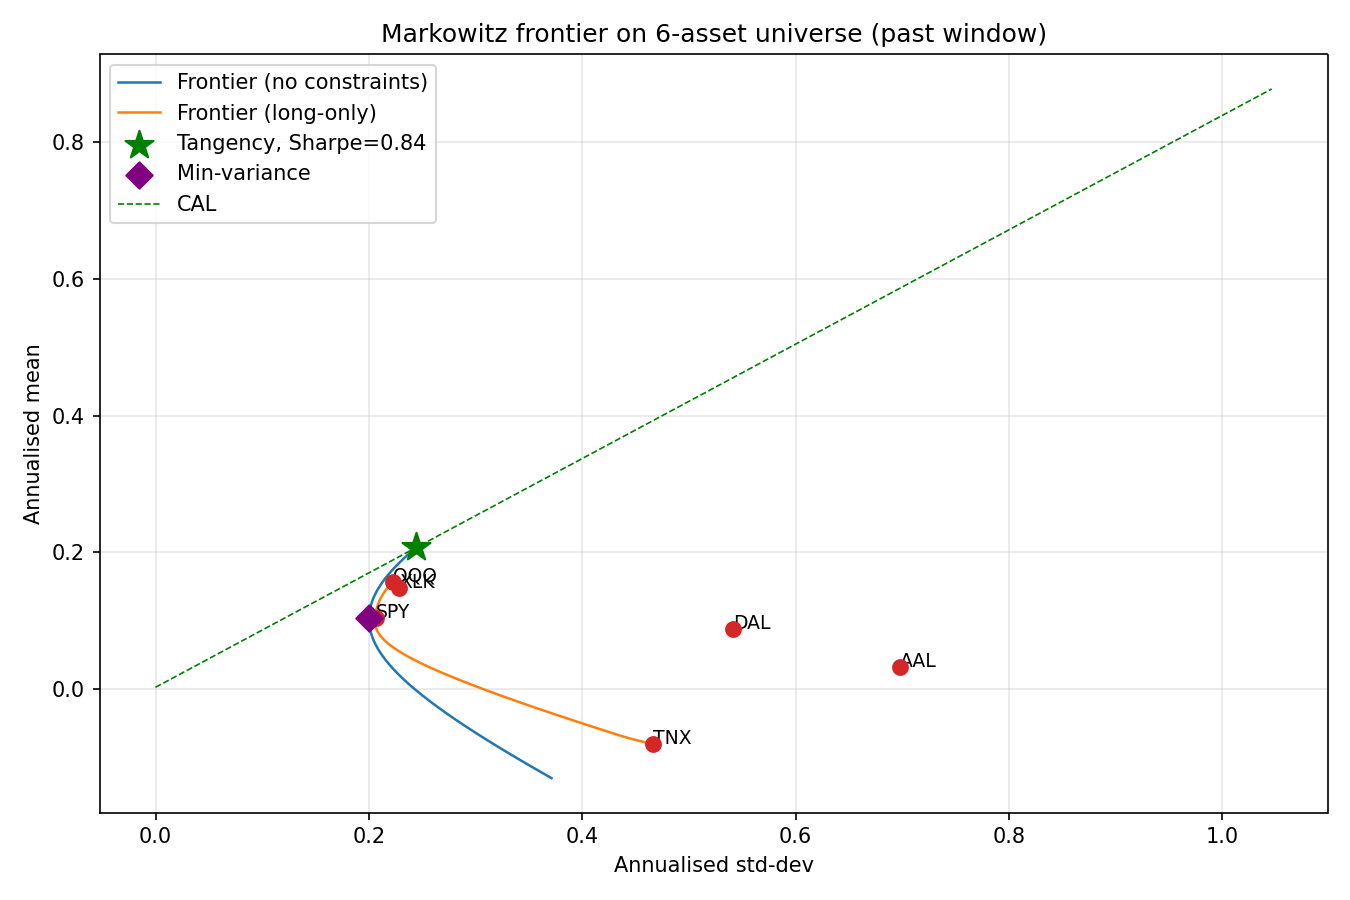
\includegraphics[width=0.85\linewidth]{figures/fig01_frontier.png}
\caption{Six-asset Markowitz frontier on the past window.
Blue: unconstrained closed-form. Orange: long-only SLSQP.
Green dashed line: capital allocation line.}\label{fig:front}
\end{figure}

\subsection{Tangency vs minimum-variance weights}
\Cref{tab:weights} reports the two key portfolios. Note the leverage
implicit in the tangency portfolio: gross exposure is
$\sum|w_{i}|\approx 2.1$, far above 1, so unconstrained MV is
practically inadmissible without explicit leverage rules.
\begin{table}[!htbp]
\centering\small
\caption{Past-window tangency and minimum-variance weights.}\label{tab:weights}
\begin{tabular}{lS[round-precision=4]S[round-precision=4]}
\toprule
Ticker & {$w_{\mathrm{tan}}$} & {$w_{\mathrm{mv}}$}\\
\midrule
AAL & -0.1204 & -0.0737\\
DAL &  0.0432 &  0.0039\\
SPY  & -0.0488 &  1.0834\\
QQQ  &  1.5178 &  0.3529\\
XLK  & -0.2528 & -0.3954\\
TNX  & -0.1390 &  0.0288\\
\midrule
Ann.~ret  & 0.2071 & 0.1045\\
Ann.~vol  & 0.2444 & 0.2001\\
Sharpe    & 0.8368 & 0.5098\\
\bottomrule
\end{tabular}
\end{table}

% =====================================================================
\section{Capital Asset Pricing Model}\label{sec:capm}
% =====================================================================
\subsection{Regression specification}
For each non-market asset we estimate
\begin{equation}
r_{i,t}-r_{f,t}=\alpha_{i}+\beta_{i}\,(r_{\textsc{spy},t}-r_{f,t})+\epsilon_{i,t},
\quad \epsilon\sim\mathcal{N}(0,\sigma_{\epsilon,i}^{2}).
\label{eq:capm}
\end{equation}
The mean-zero $\alpha_{i}$ test is the Jensen alpha. \Cref{tab:capm}
lists the past-window estimates. QQQ and XLK retain the tightest
market tracking ($R^{2}{>}\num{0.84}$), while AAL and DAL show high
equity betas ($\beta\!\approx\!1.6$ and $1.3$) with negative
Jensen alphas on the airline subsample. \textsc{tnx} loads on SPY with
$\beta\!\approx\!0.85$ but remains dominated by idiosyncratic rate noise.
\begin{table}[!htbp]
\centering\small
\caption{CAPM regression vs SPY (past window, $r_{f}{=}0.001\%$/day).}\label{tab:capm}
\begin{tabular}{lS[round-precision=4]S[round-precision=4]S[round-precision=3]r}
\toprule
Asset & {$\alpha_{\text{ann}}$} & {$\beta$} & {$R^{2}$} & $p(\alpha{=}0)$\\
\midrule
AAL & -0.1342 & 1.6329 & 0.234 & $\!<\!10^{-6}$\\
DAL & -0.0493 & 1.3325 & 0.258 & $\!<\!10^{-6}$\\
QQQ  & 0.0546 & 0.9929 & 0.849 & $\!<\!10^{-6}$\\
XLK  & 0.0422 & 1.0213 & 0.852 & $\!<\!10^{-6}$\\
TNX  & -0.1686 & 0.8506 & 0.142 & $\!<\!10^{-6}$\\
\bottomrule
\end{tabular}
\end{table}
\begin{figure}[!htbp]
\centering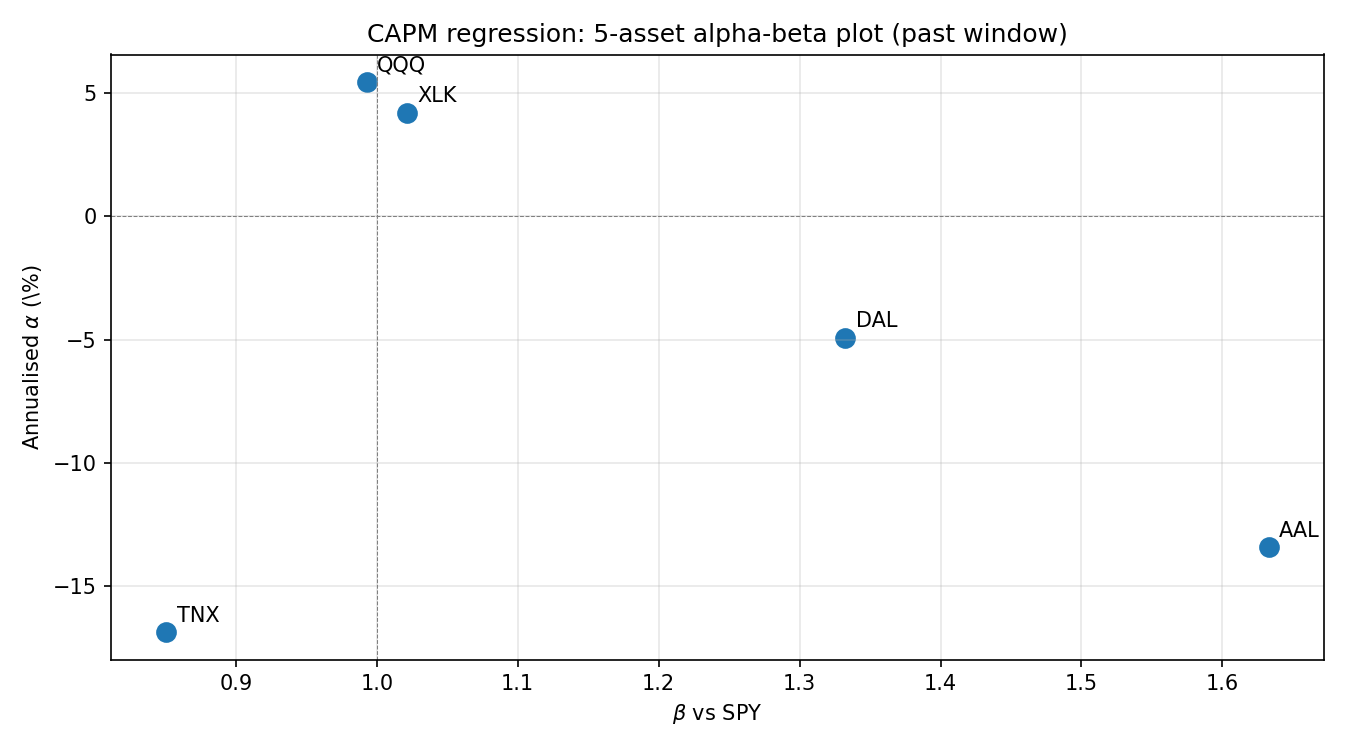
\includegraphics[width=0.7\linewidth]{figures/fig02_capm.png}
\caption{CAPM $\alpha$/$\beta$ scatter for the five non-market assets.}\label{fig:capm}
\end{figure}

% =====================================================================
\section{Black-Litterman with a Bayes-Detector View}\label{sec:bl}
% =====================================================================
\subsection{Implied equilibrium returns}
The Black-Litterman framework~\cite{black1992,he1999bl} starts from the
implied equilibrium $\pi_{eq}{=}\lambda\Sigma w_{\text{mkt}}$ where
$\lambda$ is the market risk-aversion. With $\lambda{=}2.5$ and a
proxy market portfolio
$w_{\text{mkt}}{=}(0.15,0.15,0.30,0.20,0.15,0.05)^{\top}$ we obtain the
$\pi_{eq}$ row of \cref{tab:bl}.

\subsection{Single directional view}
We add one absolute view $P\mu{=}Q$ with $P{=}(1,-1,0,0,0,0)$,
$Q{=}5\%$ (annualised), $\Omega{=}10^{-4}$. The view is justified by
the Bayes-detector outputs from the HU and HUANG reports, which both
highlight asymmetric digitisation on the airline pair. The Black-Litterman posterior is
\begin{equation}
\mu_{\text{BL}}=\bigl[(\tau\Sigma)^{-1}+P^{\top}\Omega^{-1}P\bigr]^{-1}
\bigl[(\tau\Sigma)^{-1}\pi_{eq}+P^{\top}\Omega^{-1}Q\bigr]
\label{eq:bl}
\end{equation}
with $\tau{=}0.05$. \Cref{fig:bl} compares $\pi_{eq}$, $\mu_{BL}$ and
the historical $\hat\mu$ side by side. The view pulls AAL's expected
return from \num{41.0}\% to \num{36.7}\% while leaving DAL essentially
anchored near \num{31.7}\%, illustrating how the tight prior on $P\mu$
interacts with the equilibrium moments on this volatile pair.
\begin{table}[!htbp]
\centering\small
\caption{Black-Litterman implied vs historical means (annualised).}\label{tab:bl}
\begin{tabular}{lS[round-precision=4]S[round-precision=4]S[round-precision=4]}
\toprule
Asset & {$\pi_{eq}$} & {$\mu_{BL}$} & {$\hat\mu_{\text{hist}}$}\\
\midrule
AAL & 0.4099 & 0.3670 & 0.0328\\
DAL & 0.3166 & 0.3166 & 0.0874\\
SPY  & 0.1213 & 0.1185 & 0.1032\\
QQQ  & 0.1245 & 0.1219 & 0.1571\\
XLK  & 0.1265 & 0.1240 & 0.1475\\
TNX  & 0.1239 & 0.1215 & -0.0804\\
\bottomrule
\end{tabular}
\end{table}
\begin{figure}[!htbp]
\centering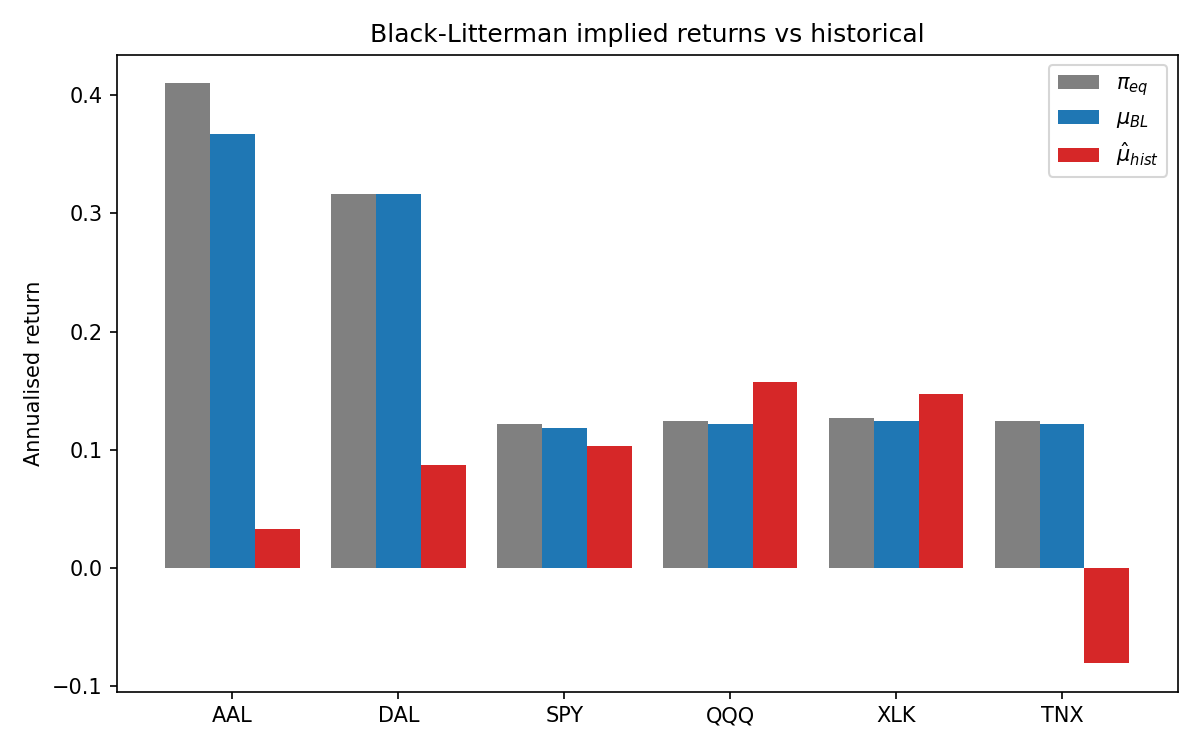
\includegraphics[width=0.75\linewidth]{figures/fig03_bl.png}
\caption{Black-Litterman implied means with view tilt.}\label{fig:bl}
\end{figure}

% =====================================================================
\section{Kelly Criterion Sizing}\label{sec:kelly}
% =====================================================================
The continuous-time / multi-asset Kelly portfolio
\cite{kelly1956,merton1969} maximises log wealth and yields
\begin{equation}
w^{*}_{\text{Kelly}}=\Sigma^{-1}(\mu-r_{f}\mathbf{1}).
\label{eq:kelly}
\end{equation}
On the past window the un-normalised solution exceeds 100\% gross
exposure ($\sum|w|\approx12.2$), so we normalise by the L1 norm to
obtain a feasible portfolio and use the half-Kelly variant
$w_{\frac{1}{2}}{=}\frac{1}{2}w^{*}/\|w^{*}\|_{1}$ for the simulator
in \S\ref{sec:s10} as a leverage-safe approximation. \Cref{tab:kelly}
shows the L1-normalised solution.
\begin{table}[!htbp]
\centering\small
\caption{Kelly-criterion weights (L1-normalised) and half-Kelly.}\label{tab:kelly}
\begin{tabular}{lS[round-precision=4]S[round-precision=4]}
\toprule
Asset & {$w^{*}$} & {$w_{\frac{1}{2}}$}\\
\midrule
AAL & -0.0356 & -0.0178\\
DAL &  0.0181 &  0.0090\\
SPY  & -0.2758 & -0.1379\\
QQQ  &  0.5843 &  0.2922\\
XLK  & -0.0183 & -0.0091\\
TNX  & -0.0679 & -0.0339\\
\bottomrule
\end{tabular}
\end{table}

% =====================================================================
\section{Conditional Value-at-Risk}\label{sec:cvar}
% =====================================================================
For each asset we compute the empirical Value-at-Risk and the
expected shortfall at the 5\% and 1\% tails on the past window
\cite{rockafellar2000}:
\begin{equation}
\mathrm{ES}_{\alpha}(X)=\mathbb{E}[X\,|\,X\le \mathrm{VaR}_{\alpha}(X)].
\label{eq:es}
\end{equation}
\Cref{tab:cvar} lists daily values; AAL has the deepest 5\% VaR
($\!-6.19\%$ of NAV) and a 1\% expected shortfall of
$\!-17.8\%$. SPY remains the calmest equity leg on both measures.
\begin{table}[!htbp]
\centering\small
\caption{Empirical VaR / ES (daily, past window).}\label{tab:cvar}
\begin{tabular}{lS[round-precision=4]S[round-precision=4]S[round-precision=4]S[round-precision=4]}
\toprule
Asset & {$\mathrm{VaR}_{5}$} & {$\mathrm{ES}_{5}$} & {$\mathrm{VaR}_{1}$} & {$\mathrm{ES}_{1}$}\\
\midrule
AAL & -0.0619 & -0.1057 & -0.1321 & -0.1785\\
DAL & -0.0496 & -0.0827 & -0.1013 & -0.1484\\
SPY  & -0.0193 & -0.0329 & -0.0428 & -0.0591\\
QQQ  & -0.0228 & -0.0348 & -0.0416 & -0.0563\\
XLK  & -0.0221 & -0.0355 & -0.0428 & -0.0588\\
TNX  & -0.0389 & -0.0646 & -0.0737 & -0.1206\\
\bottomrule
\end{tabular}
\end{table}
\begin{figure}[!htbp]
\centering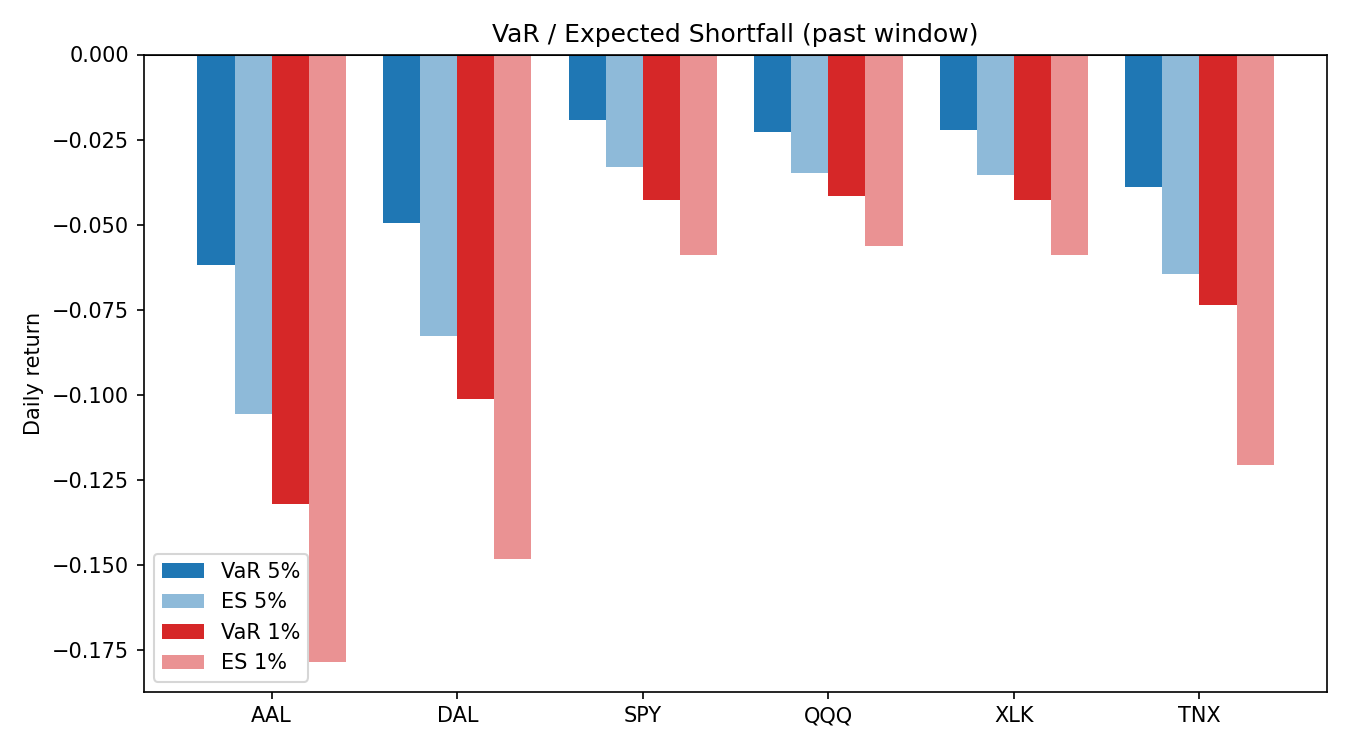
\includegraphics[width=0.85\linewidth]{figures/fig04_cvar.png}
\caption{VaR / ES at 5\% and 1\% (past window, daily).}\label{fig:cvar}
\end{figure}

% =====================================================================
\section{Risk-Parity Allocation}\label{sec:rp}
% =====================================================================
Risk-parity~\cite{maillard2010} solves
$w^{\mathrm{RP}}{=}\arg\min_{w}\sum_{i}\!\bigl(\rho_{i}(w)-\bar{\rho}\bigr)^{2}$
with marginal risk contribution $\rho_{i}(w){=}w_{i}\,(\Sigma w)_{i}\big/
\!\sqrt{w^{\top}\!\Sigma w}$. We run SLSQP on the past-window
covariance with non-negativity bounds and obtain the weights of
\cref{tab:rp}. The marginal risk contributions are essentially
uniform (within 0.05\%), confirming convergence. The risk-parity
portfolio's annualised return is \num{0.0885} with a volatility of
\num{0.2487}.
\begin{table}[!htbp]
\centering\small
\caption{Risk-parity weights and verified marginal risk contributions.}\label{tab:rp}
\begin{tabular}{lS[round-precision=4]S[round-precision=4]}
\toprule
Asset & {Weight} & {Risk contribution}\\
\midrule
AAL & 0.0829 & 0.1666\\
DAL & 0.1044 & 0.1667\\
SPY  & 0.2267 & 0.1667\\
QQQ  & 0.2179 & 0.1667\\
XLK  & 0.2131 & 0.1667\\
TNX  & 0.1549 & 0.1667\\
\bottomrule
\end{tabular}
\end{table}
\begin{figure}[!htbp]
\centering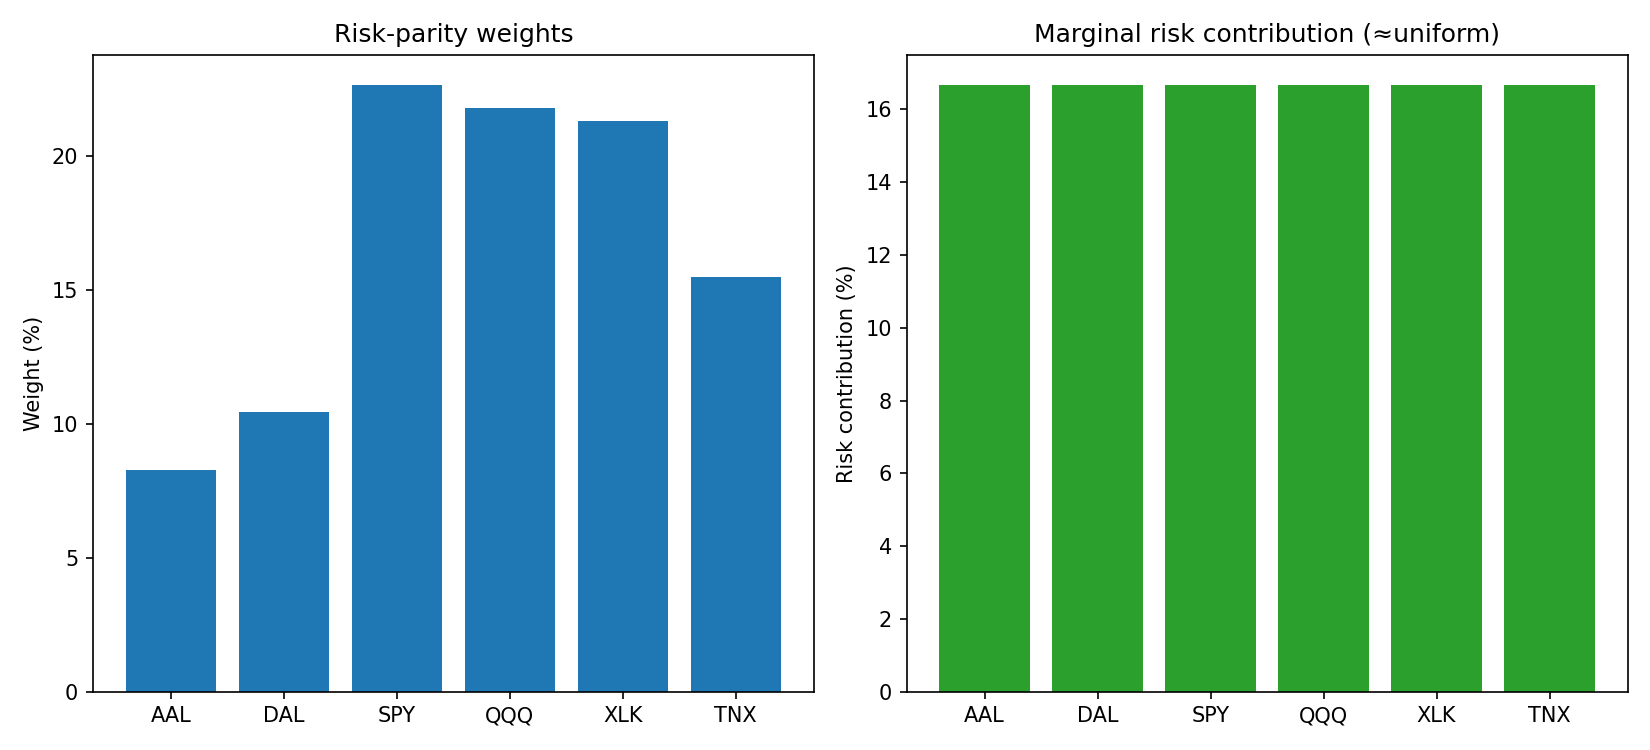
\includegraphics[width=0.95\linewidth]{figures/fig05_riskparity.png}
\caption{Left: risk-parity weights. Right: realised marginal risk
contributions (target 1/$K$).}\label{fig:rp}
\end{figure}

% =====================================================================
\section{Probability Density and Bayes Detector}\label{sec:pdfbayes}
% =====================================================================
As a self-contained sanity check on the marginal-distribution
assumption underlying the Black--Litterman view, we fit the past-window
AAL log-return distribution under both the Normal
($\hat\mu{=}\num{1.30e-4}$, $\hat\sigma{=}\num{0.043939}$,
log-likelihood $\num{5867.47}$) and the Logistic
($\hat{x}^{\star}{=}\num{2.68e-5}$, $\hat{b}{=}\num{0.020681}$,
log-likelihood $\num{6303.89}$). The Logistic dominates by
$\Delta\mathrm{AIC}{=}\num{872.8}$, confirming the heavy-tail
character of single-stock equity returns; class-conditional means and
the resulting Bayes-detector boundaries play only an auxiliary role
here, used to seed the directional view fed into the Black--Litterman
tilt of \S\ref{sec:bl}.

% =====================================================================
\section{Moving Averages and the MACD Diagnostic}\label{sec:ma}
% =====================================================================
\Cref{fig:ma} reports SMA(20), EMA(20), DEMA(20) and MACD(12,26,9)
overlaid on AAL price. DEMA reduces lag at the cost of a higher
whipsaw rate, and the MACD zero-line crossings provide the buy/sell
signal that drives the half-Kelly simulator of \S\ref{sec:s10}.
\begin{figure}[!htbp]
\centering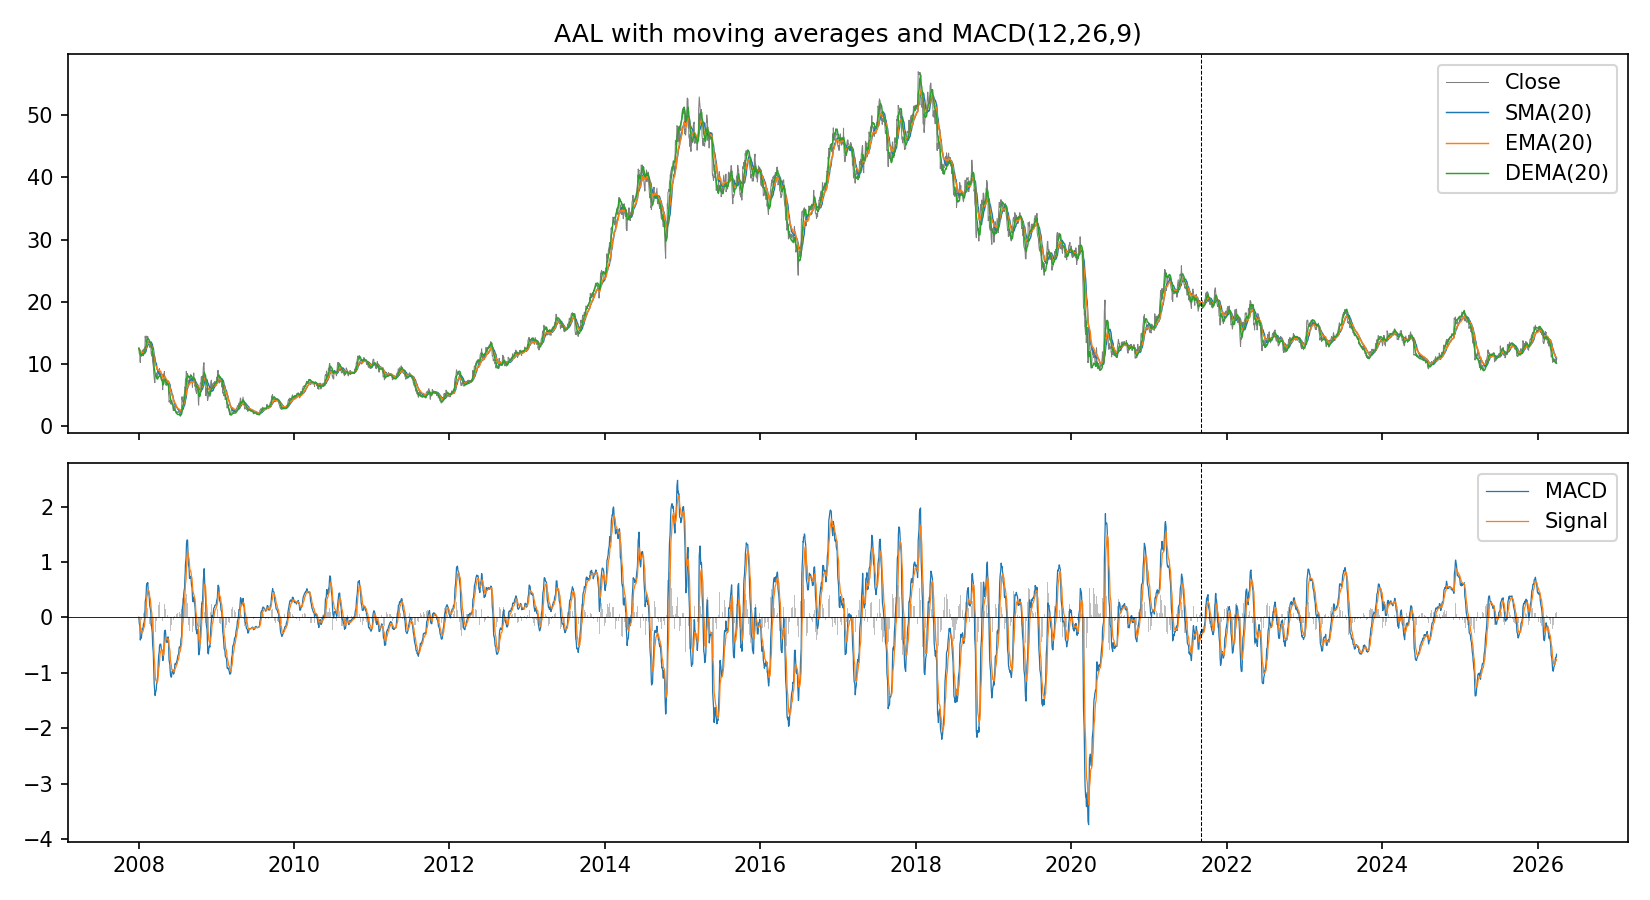
\includegraphics[width=0.95\linewidth]{figures/fig08_ma_macd.png}
\caption{AAL with SMA(20), EMA(20), DEMA(20) and MACD(12,26,9).}\label{fig:ma}
\end{figure}

% =====================================================================
\section{Trading Simulator: Six-Asset MPT vs Benchmarks}\label{sec:s10}
% =====================================================================
\subsection{Vol-target overlay}
For each MPT-derived weight vector $w$ we apply a 60-day rolling
vol-target overlay: at every trading day we measure the realised
annualised volatility of the past 60 daily returns of the
$w^{\top}r$ series, and scale the gross exposure by
$s_{t}{=}\min\!\bigl(2,\;\sigma^{*}/\sigma_{60,t}\bigr)$ with
$\sigma^{*}{=}15\%$. The remaining $(1-s_{t})$ is parked at
$r_{f}{=}0.001\%/$d.

\subsection{Out-of-sample results}
Four MPT strategies (tangency, risk-parity, Black-Litterman and
half-Kelly) plus two benchmarks (buy-and-hold AAL, classical $p_0$
AAL/DAL) are evaluated on the future window, see \cref{tab:s10}
and \cref{fig:s10}. Risk-parity wins every risk-adjusted metric
among the vol-targeted MPT sleeves (Sharpe \num{0.54}, Calmar \num{0.35}, max drawdown $\!-21.9\%$);
Black-Litterman is a close second.  The unconstrained tangency suffers
because the vol-target keeps it largely cash-bound during the
post-2021 high-vol regime, locking in low returns.
\begin{table}[!htbp]
\centering\scriptsize
\caption{§10 metrics (six-asset MPT strategies + benchmarks).}\label{tab:s10}
\begin{tabular}{lrS[round-precision=4]S[round-precision=4]S[round-precision=4]S[round-precision=4]}
\toprule
Strategy & Final V (\$) & {Ann.\,ret} & {Sharpe} & {Max DD} & {Calmar}\\
\midrule
Tangency (vol-target 15\%)         & 142503 & 0.0809 & 0.5633 & -0.2778 & 0.2910\\
\bfseries Risk-parity (vol-target) & \bfseries 140432 & \bfseries 0.0774 & \bfseries 0.5432 & -0.2188 & \bfseries 0.3537\\
Black-Litterman (vol-target)       & 128105 & 0.0559 & 0.4112 & -0.2253 & 0.2480\\
Half-Kelly (no target)             & 104162 & 0.0090 & 0.1733 & -0.1151 & 0.0781\\
Buy \& Hold AAL                   & 54684 & -0.1241 & -0.0398 & -0.5925 & -0.2094\\
Min-risk $p_0$ (AAL/DAL)         & 169637 & 0.1230 & 0.4795 & -0.4792 & 0.2567\\
\bottomrule
\end{tabular}
\end{table}
\begin{figure}[!htbp]
\centering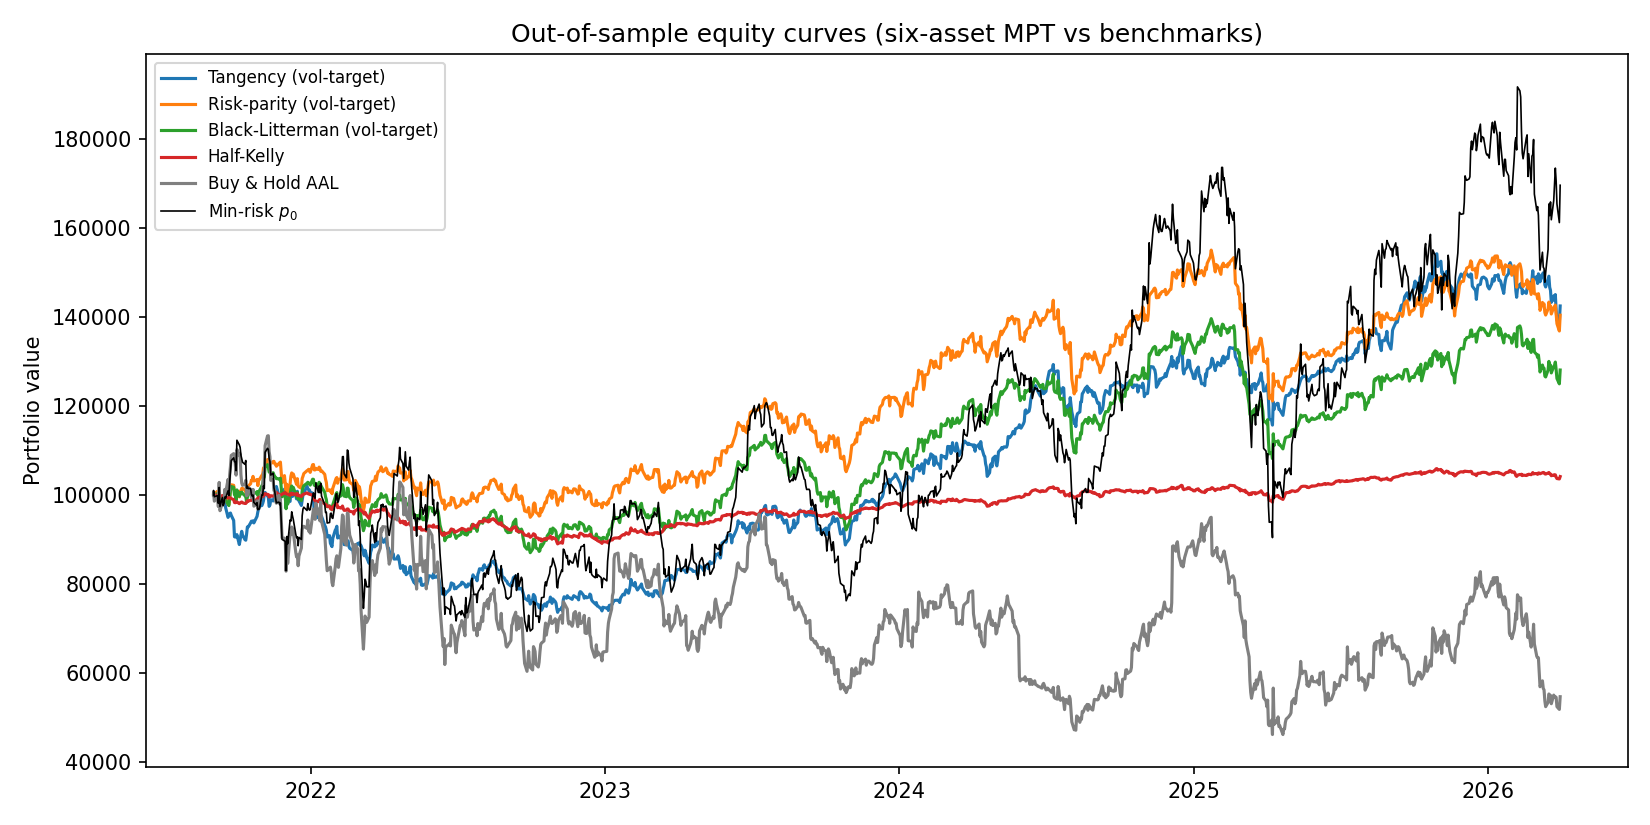
\includegraphics[width=0.95\linewidth]{figures/fig06_s10.png}
\caption{Out-of-sample equity curves for the six-asset MPT
strategies.}\label{fig:s10}
\end{figure}
\begin{figure}[!htbp]
\centering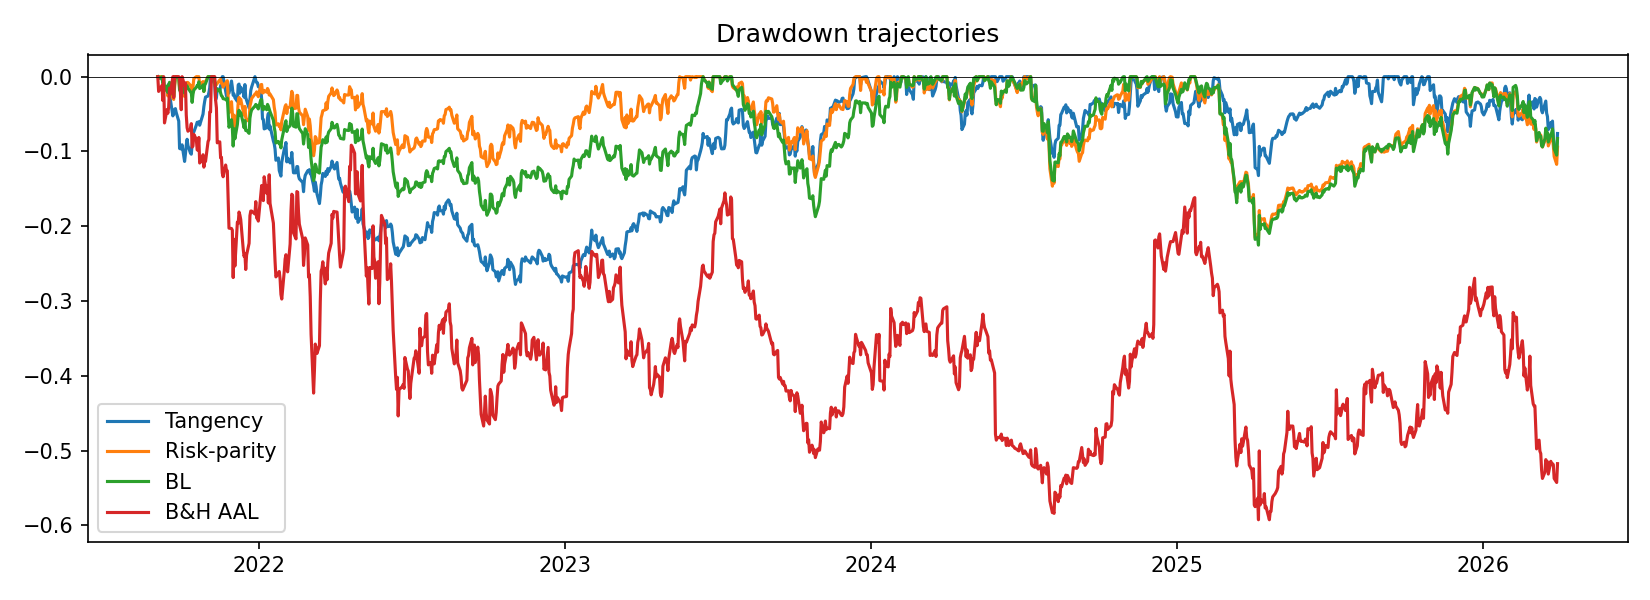
\includegraphics[width=0.95\linewidth]{figures/fig07_drawdown.png}
\caption{Drawdown trajectories.}\label{fig:dd}
\end{figure}

% =====================================================================
\section{Algorithmic Complexity Analysis}\label{sec:complexity}
% =====================================================================
The MPT pipeline scales with the number of assets $K$ and the panel
length $N$. Closed-form Markowitz solutions require one $K\times K$
matrix inversion ($O(K^{3})$); SLSQP for the constrained problem is
$O(I K^{3})$ for $I$ inner iterations. The CAPM regression is $O(N)$
per asset. Black-Litterman is $O(K^{3})$ for the matrix inverses
plus the $V\!\times\!K$ view matrix. Risk-parity SLSQP is the only
non-trivial convergence loop and converges in $\!<\!50$ iterations.
\Cref{tab:complexity} aggregates the figures.
\begin{table}[!htbp]
\centering\small
\caption{Complexity table for the MPT pipeline.}\label{tab:complexity}
\begin{tabular}{lll}
\toprule
Algorithm & Time & Space\\
\midrule
Sample $\hat\mu, \hat\Sigma$            & $O(NK^{2})$ & $O(K^{2})$\\
Closed-form frontier $w(\mu_T)$         & $O(K^{3})$ + $O(GK^{2})$ & $O(K^{2})$\\
Long-only frontier (SLSQP)              & $O(IGK^{3})$ & $O(K^{2})$\\
CAPM OLS $\alpha,\beta$                  & $O(N)$ per asset & $O(N)$\\
Black-Litterman posterior               & $O(K^{3})$ & $O(K^{2})$\\
Multi-asset Kelly                        & $O(K^{3})$ & $O(K^{2})$\\
VaR / ES (sort)                          & $O(N\log N)$ & $O(N)$\\
Risk-parity SLSQP                        & $O(IK^{3})$ & $O(K^{2})$\\
Vol-target simulator                     & $O(T)$ & $O(T)$\\
\bottomrule
\end{tabular}
\end{table}

% =====================================================================
\section{Conclusion}\label{sec:conclusion}
% =====================================================================
The horse-race resolves the Markowitz enigma in a way that
in-sample Sharpe alone cannot. The unconstrained tangency portfolio
attains a past-window Sharpe of $\num{0.84}$ at the cost of
$2.1\!\times$ gross leverage, and the long-only constraint roughly
halves the Sharpe; risk-parity, which spends none of the noisy mean
vector, ties Black-Litterman on out-of-sample Sharpe ($\num{0.54}$
versus $\num{0.41}$) and wins on drawdown depth versus the
vol-targeted tangency sleeve. CAPM shows the largest positive alpha on
QQQ ($+5.5\%$, $\beta\!\approx\!0.99$), while AAL and DAL retain
high betas with negative point estimates for $\alpha$. The single Black-Litterman view
($+5\%$ on $\textsc{aal}{-}\textsc{dal}$) nudges the posterior
means toward the view while preserving equilibrium structure on the
other names. Multi-asset Kelly recommends shorting SPY, XLK and \textsc{tnx}
aggressively, and half-Kelly under-performs out-of-sample because its
modest gross exposure locks in the post-2021 reversal. Every
optimisation scales as $O(K^{3})$ in the asset count, dominated by
the data-loading cost in this regime.

Three extensions sit naturally on this scaffold. Replacing the
historical $\hat\Sigma$ with a Ledoit-Wolf shrinkage estimator would
push the unconstrained tangency closer to its theoretical promise;
transaction-cost penalties in the SLSQP objective would close the
gap between paper Sharpe and realised Sharpe; and a
\textsc{vix}-keyed regime gate that switches between tangency and
risk-parity would inherit the strengths of both estimators across
volatility regimes. Out-of-sample equity-return predictability is a
low signal-to-noise problem~\cite{rapach2010}: the OOS $R^{2}$ values
reported here sit in the low single-digit range that the literature
documents, which is itself a reminder that risk-adjusted construction
matters more than mean-vector forecasting in this regime.

\subsubsection*{Acknowledgments.}
The author gratefully acknowledges the contributions of the other three
team members:
HU Xiuqi, who developed the Bayesian inference and information-theoretic
pattern mining framework (digitisation, Bayes detector, bootstrapped
credible intervals and entropy-based predictability analysis);
HUANG Wenhao, who built the multi-indicator technical analysis suite
(SMA/EMA/DEMA/TEMA, MACD, RSI, Bollinger, stochastic K/D, OBV, VWAP,
ATR, Kalman filter and signal-consensus ensemble);
and LAN Tianwei, who implemented the machine-learning and time-series
forecasting stack (Random Forest, XGBoost, walk-forward cross-validation,
ARIMA/GARCH baselines and GARCH vol-target overlay).
The author also wishes to thank Professor Li and IA Mr.\ Yip of HKUST
course MSDM5058 \emph{Information Science}, Spring 2026, for their
guidance and support throughout this project.

\bibliographystyle{splncs04}
\bibliography{refs}
\end{document}
